\begin{center}
\section{Introduction}
\end{center}

The Travelling Salesman Problem(TSP) is one of mathematics' most studied optimisation problems due to its simple problem definition and wide use case\cite{Flood1956}. The goal is to find the shortest route that visits every node exactly once. It is used in many fields and industries, as its graphing properties can be applied to various problems, leading to significant interest from both theorists and practitioners.

\begin{figure}[!ht]
    \centering
    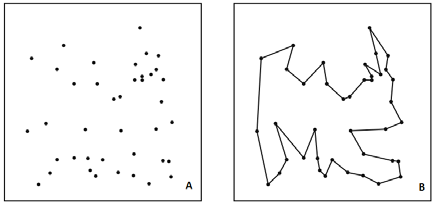
\includegraphics[width=0.9\textwidth]{sections/image/tsp.png}
    \caption{TSP And Solution}
    \cite{tsp-image}
\end{figure}

However, due to the NP-Hardness property of the problem\cite{TSP-NP-hard}, an exact solution can be computationally infeasible. Therefore, approximations are a suitable replacement for some applications where an exact solution is not required. These algorithms are called heuristics due to their approximating solutions and quick results.

Look-ahead(LA) algorithms are an algorithm design type with no formal definition. They are not a new concept, as they are primarily found in decision problems, but range from backtracking to forward checking to combinatorial search.

This report defines look-ahead as a sub-procedure that recursively checks how a greedy prediction affects future options and applies a semi-intelligent outcome with foresight. Applying foresight to avoid the common pitfalls of greedy algorithms introduces its own challenges because a look-ahead heuristic is still classified as a greedy approach; under the wrong circumstances, it will produce suboptimal results.

Dynamic look-ahead is an extension to the look-ahead algorithm design that will be explored to help resolve and improve the issues facing a standard approach to look-ahead. It aims to achieve this by changing the look-ahead search depth dynamically at runtime based on the problem at large through various metrics.

This project will apply these algorithmic designs to the existing Cheapest Insertion Heuristic(CIH) greedy algorithm to create two new algorithms, Static Look-Ahead Cheapest Insertion Heuristic and Dynamic Look-Ahead Cheapest Insertion Heuristic. Its unique design, implementation, and performance are compared to other classical algorithms and then evaluated.

An in-depth review of the Travelling Salesman Problem, existing solutions, and software optimisation techniques is conducted for the project to consider. This report researches the logical steps required to apply a look-ahead design to CIH and the potential benefits and issues that come with a look-ahead design. A scientific methodology is devised for an organised approach to the testing, evaluation, and conclusion of the findings of this project.

A significant software development project is included to verify and empirically test theoretical ideas. State-of-the-art methods and techniques are employed to ensure unbiased results and optimal performance. Algorithmic designs are coded with accuracy and are deterministic for reliability and scrutiny of the results. The same core library code is used to execute multiple runtime solutions to fit the various needs of the project. 

When evaluating a new algorithm, multiple methodologies are explored. Empirical testing on new randomly generated problems is conducted against existing conventional greedy heuristics, and then data analysis is applied. A famous testing library, TSPLib\cite{TSPLib}, of optimally solved problems serves as a ground truth to measure how the new designs perform against exact solutions.

Graphs and renders of solutions have been developed for verification and visual evidence. Allowing for easy comparison between solutions and quick data analysis is vital for later evaluations. Data collection and processing for statistics and scientific research are embedded in the analysis of each solution.

White box unit testing covered the codebase from bugs and unexpected behaviour changes. Waterfall project management helped ensure the project stayed on track and reduced the amount of refactoring and backtracking.

\subsection{Motivation}

This report will research, design, test, and evaluate the use of a look-ahead design on an existing greedy heuristic to create an improved solution over that of its greedy heuristic counterpart. This report will not attempt to solve the Travelling Salesman Problem or discuss the possibility of the P versus NP problem.

\subsection{Aims}
\label{sec:aims}

This report aims to tackle the challenges present when creating a new algorithm and to follow current research in methodology to produce a worthwhile and fair conclusion. Following this, some aims have been outlined, and each will be independently evaluated at the end of this report in Section\ref{conc:aims}.

\begin{enumerate}
  \item Design a new look-ahead algorithm that runs in polynomial time based on the greedy Cheapest Insertion Heuristic
  \item Fairly and objectively test and evaluate each performance metric of a heuristic algorithm
  \item Develop and maintain a working code base to run various algorithms reliably through a standard API
\end{enumerate}